\chapter{The API}
This chapter will explain the design and implementation of the API for this project.
\section{Design}
The API started with one clear goal, to be the middleman between the controllers and our database. The API's main purpose is to abstract away the need for the controllers to work directly with the database, along with it meaning more security for the database. With this in mind the API should also be as simple as possible, which lead to the API having only three actions. The three actions are \texttt{status}, \texttt{turn on} and \texttt{turn off}. \\
\texttt{Status}' job is a way for the controller to check up on if there have been any changes in time remaining for the user. This means that \texttt{status} has to check if there are any rules that will cut the user off before they run out of points. If there are no rules that interferes then it should calculate the time remaining again for the user and return that. \\
\texttt{Turn on}'s main function is for the controller to request for it to turn on. This means that \texttt{turn on} should check to see if the controller can be turned on, calculate the time remaining, turn on the controller inside the database and finally return that. When checking to see if the controller can be turned on, \texttt{turn on} should check both that the user has enough points for at least a minute of on time and that there are no rules that are preventing the controller from turning on.\\
\texttt{Turn off}'s main function is for the controller to tell the API that it wants to turn off. This means that \texttt{turn off} should check if it is the same user who is turning the controller off and if it is not the same user report an error. \texttt{turn off} should then calculate the time spent on the media and calculate how many points to remove from the user and then remove it. Finally it should return the time spent and the points removed.

\fixme{use figures for at least one: you can use the ones below:}

\begin{figure}
	\centering
		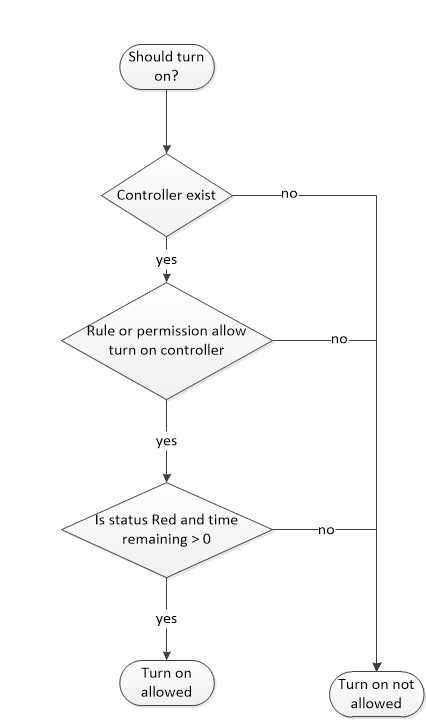
\includegraphics{images/turnOnAPI1.jpg}
	\caption{MAIN TURN ON}
	\label{fig:turnOnAPI1}
\end{figure}


\begin{figure}
	\centering
		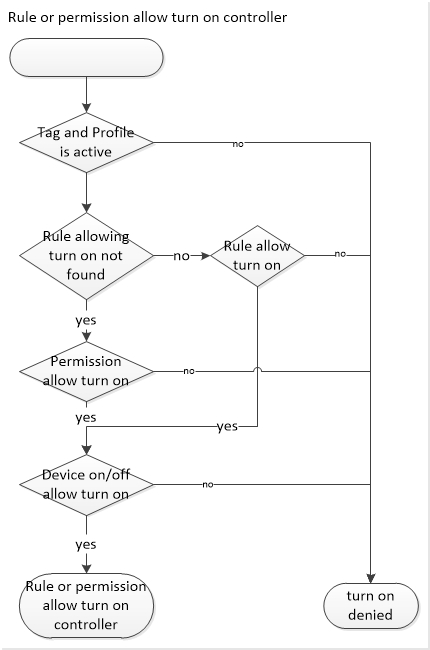
\includegraphics{images/turnOnAPI2.jpg}
	\caption{RULES ALLOW TURN ON}
	\label{fig:turnOnAPI2}
\end{figure}

 
\section{Implementation}
The API has been implemented on top of the Slim routing framework and PHP. The reason for this framework is that it makes it quicker and easier to make an API, while also making it easy to add additional endpoints. The communication between controllers and the API are done using HTTP and JSON. JSON has been chosen because of its almost universally support and its small overhead. This means that the communication is easy to implement, and easy to port to additional platforms if necessary. Calling the API is as simple as navigating to a website. Parameters to the API is done using custom GET messages. An example of a call to get status could be \texttt{http://example.com/api/api.php/turnOn/123/234} where \texttt{example.com} is the domain where the API is hosted, \texttt{123} is the controller id and \texttt{234} is the users tag id. An overview of the available calls and their parameters can be seen in \autoref{tbl:apicalls}.

\begin{table}[!h]
\begin{tabular}{| l | l | l |}
\hline
Call & Parameters & Return values \\
\hline
/status/ & cId & status, action, timeRemaining \\
\hline
/turnOn/ & cId, tId & status, timeRemaining, error \\
\hline
/turnOff/ & cId, tId & status, timeSpent, pointsRemoved, error \\
\hline
\end{tabular}
\caption{A table containing the available calls of the API. A legend of the keywords can be found in \autoref{tbl:apilegend}}
\label{tbl:apicalls}
\end{table}

\begin{table}[!h]
\begin{tabular}{| l | p{9cm} |}
\hline
Keyword & Description \\
\hline
cId & The id of a controller \\
\hline
tId & The id of a users tag \\
\hline
status & Status of the API call, \texttt{OK} if successful, \texttt{ERROR} if failure \\
\hline
action & The action the controller should take, \texttt{none} if no action should be taken \\
\hline
error & A description of the error that has occurred if any has, error is omitted from the JSON if there was no errors \\
\hline
timeRemaining & The amount of time before the controller should turn itself off in minutes \\
\hline
timeSpent & The amount of time the controller was one in minutes \\
\hline
pointsRemoved & The amount of points removed from the user \\
\hline
\end{tabular}
\caption{A table containing a legend of the keywords used in \autoref{tbl:apicalls}}
\label{tbl:apilegend}
\end{table}
